%
% File: chap02.tex
%
\let\textcircled=\pgftextcircled
\chapter{Proposed solution (Graph Partitioning for Large Graphs)}
\label{Chapter3}
GNNs aim at learning node
representations by learning the similarities shared between
connected nodes. However, the expressive ability of a GNN
is highly dependent on the quality of node features
Mention here: Deep Fraud Detection on Non-attributed Graph
https://arxiv.org/pdf/2110.01171.pdf
but cited here
C. T. Duong, T. D. Hoang, H. T. H. Dang, Q. V. H. Nguyen, and
K. Aberer, “On node features for graph neural networks,” arXiv preprint
arXiv:1911.08795, 2019.
[11] H. Cui, Z. Lu, P. Li, and C. Yang, “On positional and structural node
features for graph neural networks on non-attributed graphs,” arXiv
preprint arXiv:2107.01495, 2021

Eigendecomposition and top-k-eigenvalues are the k-dimensional feature vector
Q. Huang, H. He, A. Singh, S.-N. Lim, and A. R. Benson, “Combining
label propagation and simple models out-performs graph neural net-
works,” arXiv preprint arXiv:2010.13993, 2020.

Different feature initializations
http://www.cs.emory.edu/~jyang71/files/gnnfeature.pdf

\begin{center}
    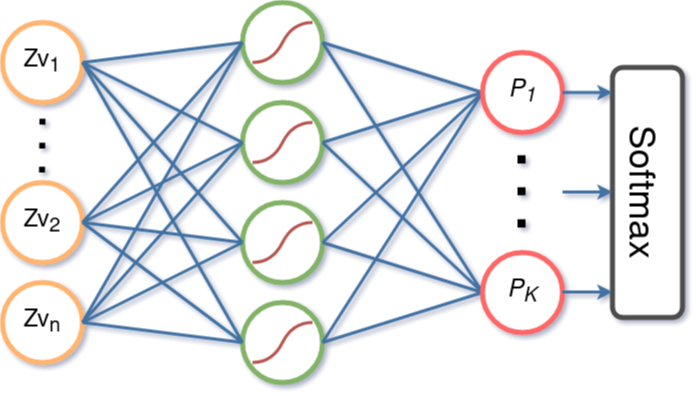
\includegraphics[scale=0.5]{partitioning_module}
\end{center}